\documentclass{article}
\usepackage[utf8]{inputenc}
\usepackage{booktabs}
\usepackage{float}
\usepackage{enumitem}
\usepackage{pgfplots}

\title{Computational Intelligence Solution for Market Pricing}
\author{Edward Evans}
\date{November 2018}

\begin{document}

\maketitle

\section{Introduction}

This paper will try to disprove the hypothesis:
\begin{quote}
"The Particle Swarm Optimization (PSO) algorithm, on average, does not perform better than the Artificial Immune System (AIS) algorithm when given the market pricing problem in terms of revenue."
\end{quote}

As a result of disproving that statement, this paper will try to prove:
\begin{quote}
"The Particle Swarm Optimization (PSO) algorithm, on average, does perform better than the Artificial Immune System (AIS) algorithm when given the market pricing problem in terms of revenue."
\end{quote}

To do so each algorithm will be implemented and run multiple times on a selection of different seeds. The revenues collected from each execution will then be compared against the opposing algorithm's results. These results will determine if the above hypotheses are true.

\section{Artificial Immune System}
\subsection{Method}

The Artificial Immune System (AIS) algorithm can solve hard problems by mimicking the processes that an immune system found within the body uses. AIS starts by creating an initial random population. Each member of the population, when applied to the market pricing problem, is a random price for each product, in a list.

The initial population is then cloned. The members of the cloned population are then mutated. For each member, the mutation varies based on how close to the optimal revenue that member is. If a member is far away from the best revenue, more of the prices are then changed.

After the mutations, the best members are selected to continue to the next iteration. The worst members are replaced with new random solutions. The steps, after and including the cloning step, are then repeated until the time allowed for execution is completed.

\subsection{Improvements}

To improve AIS some parameters can be tuned, to maximise the revenue for selected random seeds. For AIS there are four values that can be altered, the clone factor size, population size, replacement size and best fitness. To find the best values for each of these, AIS is run with the same selection of seeds each time only changing one of the parameters. The value for each of these parameters that returns the highest average revenue, then becomes the optimal parameter value. For example, in table \ref{AIS-Clone-Factor-Size}, the highest average revenue seen is 5087.223 and is given by a clone factor size of 4.

\begin{table}[h]
\begin{minipage}[b]{0.45\linewidth}
\centering
\begin{tabular}{@{}ll@{}}
\toprule
Clone Factor Size & Avg. Revenue      \\ \midrule
1                 & 5068.4065         \\
2                 & 5088.559          \\
3                 & 5064.6615         \\
4                 & 5087.223          \\
5                 & 5054.092          \\
6                 & 5052.047          \\
7                 & 5059.9535         \\
8                 & 5068.1345         \\
20                & 5020.7795         \\
50                & 4978.6845         \\
100               & 4930.1405         \\ \bottomrule
\end{tabular}
\caption{A table showing how the clone factor size affects the average revenue of the Artificial Immune System algorithm}
\label{AIS-Clone-Factor-Size}
\end{minipage}
\hfill
\begin{minipage}[b]{0.45\linewidth}
\centering
\begin{tabular}{@{}ll@{}}
\toprule
Population Size & Avg. Revenue     \\ \midrule
3               & 5085.687         \\
4               & 5094.63649999999 \\
5               & 5082.489         \\
6               & 5078.117         \\
10              & 5015.176         \\
15              & 5024.93949999999 \\
20              & 5046.69399999999 \\
25              & 4986.696         \\
30              & 5045.11799999999 \\ \bottomrule
\end{tabular}
\caption{A table showing how the population size affects the average revenue of the Artificial Immune System algorithm}
\label{AIS-Population-Size}
\end{minipage}
\end{table}


\begin{table}[h]
\begin{minipage}[b]{0.45\linewidth}
\centering
\begin{tabular}{@{}ll@{}}
\toprule
Replacement Size  & Avg. Revenue      \\ \midrule
1                 & 5092.4515         \\
2                 & 5124.686          \\
3                 & 5114.244          \\
4                 & 3506.6665         \\ \bottomrule
\end{tabular}
\caption{A table showing how the replacement size affects the average revenue of the Artificial Immune System algorithm}
\label{AIS-Best-Fitness}
\end{minipage}
\hfill
\begin{minipage}[b]{0.45\linewidth}
\centering
\begin{tabular}{@{}ll@{}}
\toprule
Best Fitness      & Avg. Revenue      \\ \midrule
5000              & 5082.1465         \\
5250              & 5128.714          \\
5500              & 5103.8535         \\
5750              & 5117.8855         \\
6000              & 5091.116          \\
7000              & 5072.9555         \\
8000              & 5094.6365         \\ \bottomrule
\end{tabular}
\caption{A table showing how the best fitness given affects the average revenue of the Artificial Immune System algorithm}
\label{AIS-Best-Fitness}
\end{minipage}
\end{table}

After completing the optimisations for each parameter in AIS, the optimal values for this set of seeds are:
\begin{itemize}[label={}]
  \item Clone Size Factor: 2
  \item Population Size: 4
  \item Replacement Size: 2
  \item Best Fitness: 5250
\end{itemize}

\section{Particle Swarm Optimization}
\subsection{Method}

The Particle Swarm Optimisation algorithm (PSO) can be used on continuous problems. PSO starts by creating a random population of particles. A particle contains a solution to the problem and other details, such as a velocity and its previous best solution.

With each iteration, the best solution within the population is found. Each particle then has its velocity calculated based on inertia, its previous best solution and the best solution found by the entire population. Then each particle's solution is changed  by applying the velocity calculated. This results in each particle swarming around the best solution, in the hope a particle finds a better solution to the problem.

\subsection{Improvements}

PSO can be optimised by changing the population size, inertia, the cognitive coefficient and social coefficient. To find the best value for each of theses parameters, only the parameter wanting to be improved is changed whilst the rest of the parameters remain the same. After trialing a set of values for the parameter, the one which returns the highest average revenue is used.

\begin{table}[h]
\begin{minipage}[b]{0.45\linewidth}
\centering
\begin{tabular}{@{}ll@{}}
\toprule
Population Size   & Avg. Revenue      \\ \midrule
100               & 5645.2315         \\
200               & 5707.546          \\
300               & 5777.8645         \\
400               & 5788.269          \\
500               & 5763.8675         \\
600               & 5824.505          \\
700               & 5825.435          \\
800               & 5841.489          \\
900               & 5826.2565         \\
1000              & 5835.1            \\
2000              & 5853.6085         \\ \bottomrule
\end{tabular}
\caption{A table showing how the population size affects the average revenue of the Particle Swarm Optimization algorithm}
\label{PSO-Population-Size}
\end{minipage}
\hfill
\begin{minipage}[b]{0.45\linewidth}
\centering
\begin{tabular}{@{}ll@{}}
\toprule
Inertia         & Avg. Revenue     \\ \midrule
0.1             & 55388.274        \\
0.2             & 5393.3815        \\
0.3             & 5402.6655        \\
0.4             & 5523.3715        \\
0.5             & 5599.2075        \\
0.6             & 5685.5295        \\
0.7             & 5838.55          \\
0.721           & 5866.4915        \\
0.8             & 5901.375         \\
0.9             & 5945.044         \\
1               & 4880.5175        \\ \bottomrule
\end{tabular}
\caption{A table showing how the inertia affects the average revenue of the Particle Swarm Optimization algorithm}
\label{PSO-Inertia}
\end{minipage}
\end{table}

\begin{table}[h]
\begin{minipage}[b]{0.45\linewidth}
\centering
\begin{tabular}{@{}ll@{}}
\toprule
Social Coefficient & Avg. Revenue      \\ \midrule
0.7                & 5913.1325         \\
0.8                & 5945.9055         \\
0.9                & 5940.58           \\
1.0                & 5923.2675         \\
1.1                & 5893.0075         \\
1.1193             & 5945.044          \\
1.2                & 5850.541          \\ \bottomrule
\end{tabular}
\caption{A table showing how the social coefficient affects the average revenue of the Particle Swarm Optimization algorithm}
\label{PSO-Social-Coefficient}
\end{minipage}
\hfill
\begin{minipage}[b]{0.45\linewidth}
\centering
\begin{tabular}{@{}ll@{}}
\toprule
Cognitive Coefficient & Avg. Revenue      \\ \midrule
0.7                   & 5894.6765         \\
0.8                   & 5937.2155         \\
0.9                   & 5921.913          \\
1.0                   & 5916.749          \\
1.1                   & 5910.546          \\
1.1193                & 5913.1325         \\
1.2                   & 5928.1135         \\ \bottomrule
\end{tabular}
\caption{A table showing how the cognitive coefficient affects the average revenue of the Particle Swarm Optimization algorithm}
\label{PSO-Cognitive-Coefficient}
\end{minipage}
\end{table}

After optimising the four parameters for PSO, the optimal values for the selection of seeds the algorithm are run on are as follows:
\begin{itemize}[label={}]
  \item Population Size: 2000
  \item Inertia: 0.9
  \item Cognitive Coefficient: 0.8
  \item Social Coefficient: 0.8
\end{itemize}

\section{Results}

After optimising each algorithm, they were both run with the same selection of seeds. The resulting revenues for each algorithm can be seen in table \ref{Seed-Results}. These results are then inputted into Welch’s t-test. The result gives a p-value of 0.000465. This p-value can then be compared against the significant level, which is 0.05. As the p-value is less than the significant level, the first hypothesis that PSO is no better, on average than AIS has been successfully disproved. This means that PSO does do better than AIS, on average, for the given problem set.

\begin{table}[H]
\centering
\begin{tabular}{@{}lllllllll@{}}
\toprule
Seed & PSO & AIS & Seed & PSO & AIS & Seed & PSO & AIS\\ \midrule
0	&	4850.3	&	4094.41	&	550	&	7004.77	&	5944.18	&	1100	&	8163.81	&	7002.96\\
50	&	5662.84	&	4736.69	&	600	&	5488.78	&	4317.06	&	1150	&	7257.54	&	6056.27\\
100	&	6623.14	&	5811.5	&	650	&	4531.03	&	3912.82	&	1200	&	4425.77	&	3783.32\\
150	&	6721.28	&	5766.99	&	700	&	6749.55	&	5747.99	&	1250	&	4718.91	&	3671.85\\
200	&	5299.78	&	4755.44	&	750	&	8205.17	&	7005.42	&	1300	&	5378.81	&	4437.59\\
250	&	6291.76	&	5491.72	&	800	&	5095.29	&	4467.36	&	1350	&	7106.14	&	5952.53\\
300	&	4404.94	&	3425.23	&	850	&	4333.09	&	3669.42	&	1400	&	6751.13	&	5478.17\\
350	&	6321.99	&	5508.57	&	900	&	6261.3	&	5588.94	&	1450	&	6670.19	&	5418.55\\
400	&	7054.8	&	6048.05	&	950	&	5297.22	&	4195.41	&	1500	&	8361.72	&	7382.26\\
450	&	5971.35	&	4960.98	&	1000	&	5051.75	&	4297.68	&	1550	&	4956.78	&	4087.16\\
500	&	6822.01	&	5887.2	&	1050	&	6211.78	&	5319.49	&	1600	&	5197.07	&	4238.38\\					
Avg.&6037.63&5104.8967\\\midrule
\end{tabular}
\caption{A table showing the resulting revenues of each algorithm with different random seeds}
\label{Seed-Results}
\end{table}

Figure \ref{revenues}, shows how each algorithm improves during its execution, when given the a seed of 100. It can be seen that PSO returns the highest revenue. 

When PSO starts its revenue is similar to the starting revenue of AIS. Within the first second of execution the revenue improves the most, then for the later two seconds it only makes minor improvements.

AIS follows a similar trend to PSO, improving at the beginning then improving less later in its execution. The sudden jumps in revenue may be a result of a good random solution replacing one of the worse solutions in the population.

\begin{figure}[h]
\centering

\caption{The highest revenue found throughout each algorithm's execution. (Seed: 100)}
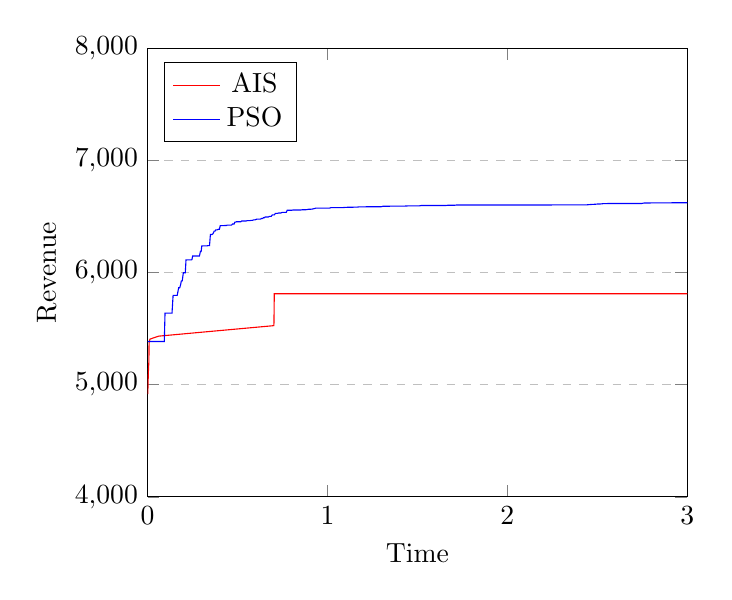
\begin{tikzpicture}
\begin{axis}[
    xlabel={Time},
    ylabel={Revenue},
    xmin=0.0, xmax=3,
    ymin=4000, ymax=8000,
    xtick={0,1,2,3},
    ytick={},
    legend pos=north west,
    ymajorgrids=true,
    grid style=dashed,
]
 
\addplot[
    color=red,
    ]
    coordinates {
    (0.0009984,4916.07)(0.0040169,5107.93)(0.0069814,5207.92)(0.0081312,5374.63)(0.0129286,5407.04)(0.0608001,5433.56)(0.7021005,5527.4)(0.7031171,5658.71)(0.7041144,5811.5)(3,5811.5)
    };

\addplot[
    color=blue,
    ]
    coordinates {
          (0,5385.36)(0.0628635,5385.36)(0.0898851,5385.36)(0.0927171,5385.36)(0.0967391,5639.26)(0.1026931,5639.26)(0.1166531,5639.26)(0.127623,5639.26)(0.1356364,5639.26)(0.1416199,5797.91)(0.145634,5797.91)(0.1506072,5797.91)(0.1567109,5797.91)(0.1645251,5797.91)(0.1725351,5865.08)(0.1785181,5865.08)(0.183509,5893.55)(0.1874662,5926.25)(0.1924826,5926.25)(0.1984662,5998.81)(0.2044185,5998.81)(0.209452,5998.81)(0.2133939,6114.23)(0.2194104,6114.23)(0.2224017,6114.23)(0.2263594,6114.23)(0.2303803,6114.23)(0.2353513,6114.23)(0.2393546,6114.23)(0.2423458,6114.23)(0.2463388,6116.55)(0.2502949,6148.43)(0.2543431,6148.43)(0.2592719,6148.43)(0.2622637,6148.43)(0.2662864,6148.43)(0.2692918,6148.43)(0.2732672,6148.43)(0.2782541,6148.43)(0.2833485,6148.43)(0.2881949,6148.43)(0.2932142,6188.63)(0.2974677,6188.63)(0.3012196,6239.11)(0.3053036,6239.11)(0.3101688,6239.11)(0.3151545,6239.11)(0.3181463,6239.11)(0.3224113,6239.11)(0.3261267,6239.11)(0.3300816,6239.11)(0.3353399,6240.81)(0.3400884,6240.81)(0.344078,6240.81)(0.3490649,6340.22)(0.3532354,6340.22)(0.3580397,6340.22)(0.3619969,6344.85)(0.3660252,6356.73)(0.3700142,6370.9)(0.3749624,6370.9)(0.3789828,6382.38)(0.3830651,6382.38)(0.386962,6382.38)(0.3909533,6385.86)(0.3949475,6387.61)(0.398899,6387.61)(0.4039195,6419.49)(0.4090213,6419.49)(0.4138813,6419.49)(0.4169061,6419.49)(0.4209651,6419.49)(0.4248603,6419.49)(0.4288522,6420.87)(0.432856,6420.87)(0.4378264,6420.87)(0.4418166,6424.61)(0.4457732,6424.61)(0.448765,6424.61)(0.4528849,6424.61)(0.4567812,6424.61)(0.461763,6424.61)(0.4667493,6424.61)(0.4717049,6434.06)(0.475694,6434.06)(0.4807275,6434.06)(0.4847023,6450.55)(0.4886902,6450.55)(0.4927874,6454.11)(0.4980894,6454.11)(0.5026565,6454.11)(0.5076081,6454.11)(0.5126274,6454.11)(0.5176541,6454.11)(0.5225687,6461.22)(0.5276182,6461.22)(0.5335591,6461.22)(0.5386774,6461.22)(0.5425481,6461.22)(0.5475333,6461.22)(0.5525208,6463.76)(0.5584719,6463.76)(0.5644902,6463.76)(0.5694424,6463.76)(0.5744634,6467.05)(0.5784524,6467.05)(0.5834058,6467.05)(0.5884512,6470.71)(0.5933778,6470.71)(0.599395,6472.36)(0.6053473,6476.87)(0.6103689,6477.48)(0.6155548,6477.48)(0.6213291,6477.48)(0.6273684,6477.48)(0.6323092,6483.17)(0.6382928,6483.17)(0.6442764,6490.05)(0.6484577,6490.05)(0.6532199,6496.49)(0.6592353,6496.49)(0.6651865,6496.49)(0.6712042,6496.49)(0.6771542,6502.34)(0.6822748,6502.34)(0.6872611,6502.34)(0.693144,6516.16)(0.6992265,6516.16)(0.705114,6516.16)(0.7101008,6528.4)(0.7160844,6528.4)(0.7220669,6529.14)(0.72905,6532.57)(0.7351382,6532.57)(0.7410211,6532.57)(0.7470263,6537.93)(0.750992,6537.93)(0.7562008,6537.93)(0.7609305,6537.93)(0.7659379,6537.93)(0.7709356,6537.93)(0.7759225,6556.83)(0.7809082,6556.83)(0.7868634,6556.83)(0.7919663,6556.83)(0.7970169,6556.83)(0.8018473,6556.83)(0.8068405,6558.95)(0.8117944,6558.95)(0.8178104,6558.95)(0.8230396,6558.95)(0.8287814,6558.95)(0.8347343,6558.95)(0.8398071,6558.95)(0.8457611,6558.95)(0.8517219,6558.95)(0.8577077,6560.85)(0.8636566,6560.85)(0.8696743,6560.85)(0.8767012,6560.85)(0.8847908,6562.42)(0.8935762,6565.32)(0.9035494,6565.46)(0.9128462,6566.86)(0.920504,6569.36)(0.9284821,6572.62)(0.9354635,6576.24)(0.9434422,6576.24)(0.950505,6576.24)(0.9564078,6576.24)(0.961468,6576.24)(0.966381,6576.24)(0.9723651,6576.24)(0.9793465,6576.24)(0.9863279,6576.24)(0.9933093,6576.24)(0.9993589,6576.24)(1.0062908,6576.24)(1.0122585,6576.24)(1.0182426,6580.1)(1.025224,6580.1)(1.0322054,6580.1)(1.0391863,6580.1)(1.045171,6580.1)(1.0511546,6580.1)(1.058136,6580.1)(1.0681092,6580.36)(1.0770857,6580.36)(1.08514,6580.36)(1.093043,6581.57)(1.1000239,6583.12)(1.1080657,6583.12)(1.1170359,6583.71)(1.1250522,6583.71)(1.1329358,6583.71)(1.1409145,6583.71)(1.1468987,6584.42)(1.1548772999999999,6584.42)(1.1629391,6584.42)(1.1718524,6586.17)(1.1798106,6587.2)(1.1877893,6587.2)(1.195768,6587.2)(1.2038177,6587.2)(1.210728,6587.2)(1.2187067,6588.52)(1.2267622,6588.52)(1.2356613,6588.52)(1.24364,6588.52)(1.2526159,6588.52)(1.2615919,6588.52)(1.2715651000000001,6588.52)(1.2815387999999999,6588.52)(1.2905148,6588.52)(1.2995533,6588.52)(1.3084666999999999,6592.52)(1.3184399,6592.52)(1.3274390999999999,6592.52)(1.3353945,6592.52)(1.3423759,6592.52)(1.3513518,6593.56)(1.3623228,6593.56)(1.372296,6593.56)(1.3823221,6593.56)(1.3932403,6593.56)(1.4022162,6593.56)(1.4131871999999999,6593.56)(1.425155,6593.56)(1.4371233,6594.99)(1.4481728,6595.45)(1.4590642,6595.45)(1.4690374,6595.45)(1.4800084,6596.2)(1.4910443,6596.2)(1.5019493000000002,6596.2)(1.5119224999999998,6596.2)(1.5208985,6599.3)(1.5308722000000001,6599.3)(1.5418427000000001,6599.3)(1.553811,6599.3)(1.5657787,6599.3)(1.5767498,6599.3)(1.5877202000000001,6599.3)(1.5987152,6599.3)(1.6096617,6599.3)(1.6216294,6599.3)(1.6346536,6599.3)(1.6466247,6599.3)(1.6585526000000002,6599.3)(1.6687676,6601.42)(1.6794747,6601.42)(1.6894485000000001,6601.42)(1.6984778999999999,6601.42)(1.7074099999999999,6601.42)(1.7173734999999999,6603.92)(1.7293418,6603.92)(1.7423636999999998,6603.92)(1.7502855,6603.92)(1.7573306,6603.92)(1.7653349,6603.92)(1.7752192999999998,6603.92)(1.7862148,6603.92)(1.7971608,6603.92)(1.8081312999999999,6603.92)(1.8161834,6603.92)(1.8240886,6603.92)(1.8330646000000002,6603.92)(1.8421213,6603.92)(1.853011,6603.92)(1.8640423,6603.92)(1.8729578999999998,6603.92)(1.8819339,6603.92)(1.8909098,6603.92)(1.9018809,6603.92)(1.9128672,6603.92)(1.9248509,6603.92)(1.9357906,6603.92)(1.9457923,6603.92)(1.9557689,6603.92)(1.9647443,6603.92)(1.974718,6603.92)(1.9856919,6603.92)(1.9976591,6603.92)(2.0076391,6603.92)(2.0185692,6603.92)(2.0286641,6603.92)(2.0395714,6603.92)(2.051513,6603.92)(2.065473,6603.92)(2.076473,6603.92)(2.0884436,6603.92)(2.0994112,6603.92)(2.1123199,6603.92)(2.1252848,6603.92)(2.1392477,6603.92)(2.15127,6603.92)(2.1642122,6603.92)(2.1781773,6603.92)(2.1941057,6603.92)(2.2080622,6603.92)(2.2210272,6603.92)(2.236063,6603.92)(2.2509838,6604.25)(2.2640449,6604.25)(2.2779139,6604.25)(2.2908783,6604.25)(2.3048047,6604.25)(2.3168692,6604.25)(2.3299206,6604.25)(2.3437002,6604.25)(2.3576625,6604.25)(2.3716583,6604.25)(2.3845909,6604.25)(2.3975894,6604.25)(2.4105544,6604.25)(2.4235205,6604.7)(2.4375977,6604.7)(2.4534072,6606.93)(2.4693958,6608.73)(2.4884951,6610.41)(2.5052688,6613.07)(2.5184818,6613.07)(2.5311982,6615.38)(2.5451622,6615.94)(2.5592155,6616.85)(2.572123,6616.85)(2.5841738,6616.85)(2.5980621,6616.85)(2.6100206999999997,6616.85)(2.6239829,6616.85)(2.639909,6616.85)(2.6558658,6616.85)(2.6718829,6616.85)(2.6868168,6616.95)(2.700746,6616.95)(2.715061,6616.95)(2.7301314,6616.99)(2.7456576,6616.99)(2.7596204,6621.44)(2.7745492,6621.44)(2.787513,6621.44)(2.7994819,6622.28)(2.8104905000000002,6622.28)(2.8244152,6622.28)(2.8363829000000003,6623.14)(2.8465086,6623.14)(2.8585548,6623.14)(2.8693279,6623.14)(2.8792948000000003,6623.14)(2.8902715,6623.14)(2.9013239,6623.14)(2.9112152,6623.14)(2.9221856,6624.24)(2.9321276,6624.24)(2.9421457,6624.24)(2.9521075,6624.24)(2.962079,6624.24)(2.9730444,6624.24)(2.9850183,6624.24)(2.9989812000000002,6624.24)(3,6624.24)
    };

\legend{AIS,PSO}
 
\end{axis}
\end{tikzpicture}
\label{revenues}
\end{figure}


\section{Conclusion}

This paper has stated the steps required to implement the Particle Swarm Optimisation algorithm and Artificial Immune System algorithm and the improvements that can be made to increase the resulting revenue for a given set of problems.

The results from each algorithm were then compared using Welch’s t-test, this gave a result lower than the significance level. Due to this result the null hypothesis
\begin{quote}
"The Particle Swarm Optimization (PSO) algorithm, on average, does not perform better than the Artificial Immune System (AIS) algorithm when given the market pricing problem in terms of revenue."
\end{quote}
can be rejected. Therefore the alternative hypothesis
\begin{quote}
"The Particle Swarm Optimization (PSO) algorithm, on average, does perform better than the Artificial Immune System (AIS) algorithm when given the market pricing problem in terms of revenue."
\end{quote}
has been proved.

\end{document}
